\chapter{Konzepte}
\label{sec:konzepte}

In diesem Kapitel werden abstrakte Konzepte beschrieben. Besonders unerfahrene Entwickler eines Online-Multiplayer Spiels sollen anhand von diesen Konzepten Ideen für eine sinnvolle Herangehensweise erhalten, um einen roten Faden in ihrer Entwicklung verfolgen zu können. Insbesondere wenn der Entwickler noch wenig oder keine Erfahrung mit der Entwicklung von Online-Mulitplayerspielen gesammelt hat, sollen diese Konzepte bei der Erstellung einer soliden Grund-Architektur nützlich sein.

Bevor eines dieser Konzepte angewandt werden kann, müssen folgende Voraussetzungen erfüllt sein:

1. Das grundsätzliche Spielkonzept steht fest.

2. Anhand von dem festgelegten Spielkonzept kann abgeschätzt werden, ob sich für das Spiel eine Client / Server oder eine Client / Host Architektur eignet.

Sollte das Team bzw. der Solo-Entwickler zum Entschluss gekommen sein, dass sich ein Client / Server Modell am besten für den spezifischen Use Case eignet, so müssen Vorkehrungen getroffen werden, um die Hardware-Ressourcen für den späteren Server-Runner bzw. die Matchmaking API sicherzustellen. Die Grundvoraussetzung ist jedoch ein aus dem Internet erreichbarer PC mit einer festen IP-Adresse. 

Alternativ kann auch zunächst lokal innerhalb eines LAN \cite{Wikipedia.2022} entwickelt werden. Hierbei ist jedoch wichtig, dass eventuell auftretende Seiteneffekte, die durch Latenz \cite{Wikipedia.2022b} oder Bandbreite \cite{Wikipedia.2019b} verursacht werden, nicht unter Realbedingungen getestet werden können. Es empfiehlt sich deshalb bereits innerhalb der ersten Entwicklungsiterationen auszutesten, wie Prototypen für Serverprozesse auf unterschiedliche Standorte der Serverhardware reagieren. 

Nun gilt es, passende Technologien zu finden. Hier gibt es keine klare Empfehlung, jedoch können die in diesem Kapitel beschriebenen Konzepte bei der Entscheidung helfen. Es gibt bereits Frameworks \& Game Engines, die manche dieser Konzepte bereits implementiert haben und als Libraries für Entwickler bereitstellen.

\cite{MFatihMAR.2021}

\section{Vorwort zu den aufgestellten Konzepten}

Wie bereits in der Einführung erläutert, sind die folgenden Konzepte keine konkrete Entwicklungsanleitung. Vielmehr sind sie im Kontext einer bereits erarbeiteten Spielidee eine Hilfestellung zur Erarbeitung einer individuellen technischen Architektur.

Konkret muss beachtet werden, dass einige der Konzepte nicht als einzelne Programm-Klassen verstanden werden müssen, sondern als Hilfestellung für Ableitungen zu konkreten Klassen oder Skripten genutzt werden können. Es ist auch gut denkbar, dass einige Implementierungen deutliche Vorteile genießen, wenn bestimmte Konzepte jeweils für getrennte Spiel-Szenen \cite{Wikipedia.2012} umgesetzt werden.

Die Konzepte sind als separat voneinander zu betrachtende Softwarekomponenten zu sehen, die miteinander kommunizieren können. Man könnte die einzelnen implementierten Konzepte auch als Microservices \cite{Thones.2015} bezeichnen, die innerhalb eines Server-Prozesses eigene interne Abläufe besitzen und durchführen. Die Kommunikation zwischen den Komponenten sollte über direkte gegenseitige Funktionsaufrufe oder über ereignisgesteuerte Funktionen \cite{Michelson.2006} geschehen.

\section{API für Matchmaking \& Server Runner}

Für Spiele, welche ein Matchmaking-System benötigen, muss eine API entworfen werden, welche unabhängig von einem existierenden Client oder Serverprozess arbeitet. Diese API hat 2 grundsätzliche Aufgaben. 

\textbf{Matchmaking:}

Die API muss einen Algorithmus implementieren, welcher mehrere Spieler zu einer Spiel-Session zusammenführt. Mögliche Matchmaking Konzepte sind bereits im Hintergrund-Kapitel beschrieben. Die Matchmaking API verwaltet als eine Liste an aktiven Serverprozessen sowie die Information, wie man sich zu ihnen verbindet. In der Regel wird pro Serverprozess ein Netzwerk-Port an der Server-Maschine reserviert, auf denen sich dann N Spieler verbinden können.

Je nach Spielkonzept können hunderte, tausende Serverprozesse existieren, welche jeweils nur eine vergleichsweise geringe Anzahl (1-20) an Spieler verwalten. Spielkonzepte, welche viele Spieler (200-1000) innerhalb eines einzigen Serverprozesses voraussetzten, erzeugen dagegen zwar quantitativ weniger Serverprozesse, diese neigen aber in der Regel schnell zu Überlastung. Neben der Umsetzung von Interest Management und einer performanten Architektur für möglichst wenig Network-Traffic kann aber auch die Matchmaking API Abhilfe schaffen, bspw. durch 'Umverlegung' von Spielern auf andere oder neue Cluster.

\textbf{Server Runner:}

Neben dem Matchmaking ist die API ebenfalls auch zuständig für das Starten und die Überwachung von Serverprozessen.
Ebenfalls können technische Statusinformationen über aktuell laufende Spiel innerhalb eines Serverprozesses von der API verwaltet werden, beispielsweise ob es möglich ist einem Server beizutreten, oder wie viele Spieler bereits auf einem Serverprozess spielen.

Die folgende Grafik visualisiert beide Aufgaben:

\begin{figure}[H]
	\centering
	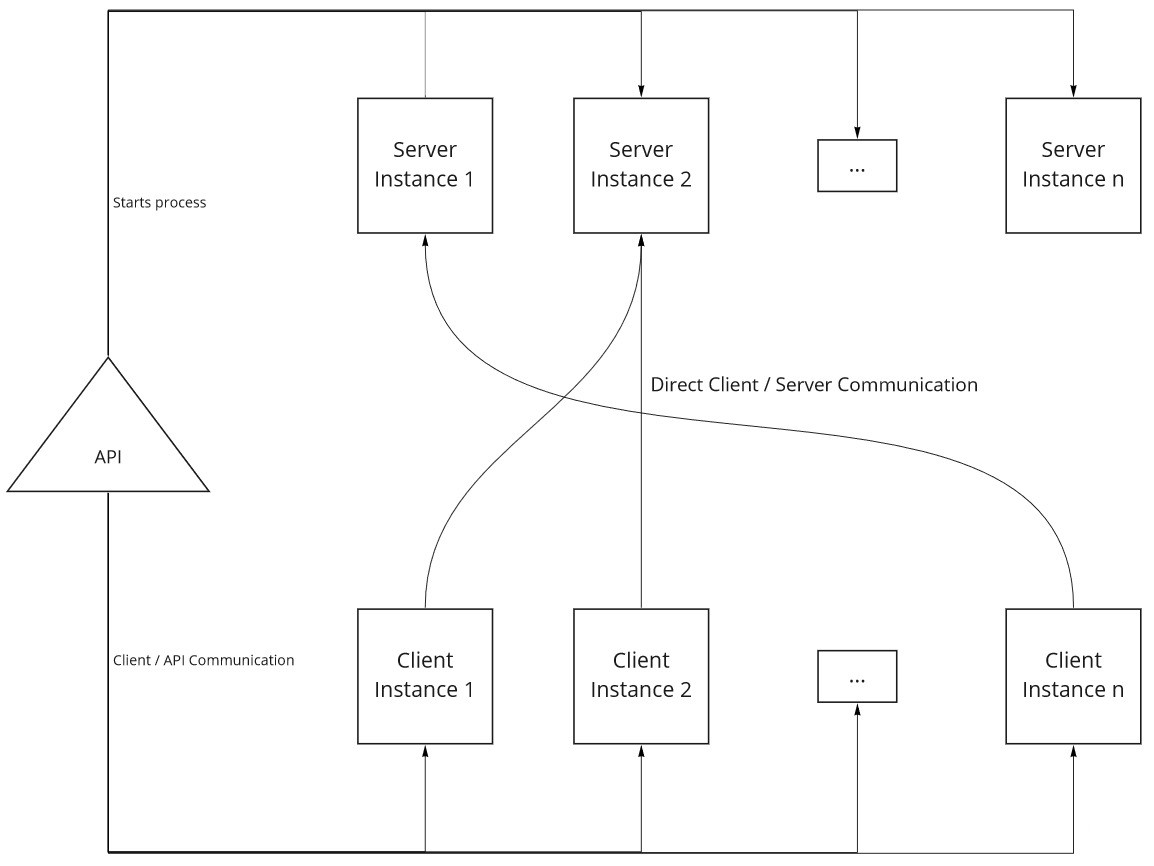
\includegraphics[width=150mm]{images/API_Konzept_Diagramm.jpg}
	\caption[API Konzept Diagramm]{Veranschaulichung des API-Konzepts}
	\label{pic:API_Konzept_Diagramm}
\end{figure}

Je nach Spiel kann das Aufgabenfeld der API um weitere Punkte erweitert werden, beispielsweise die Verwaltung einer Datenbank für Authentifizierung bzw. Kommunikation mit externen Authentifizierungs-Service-Providern oder für einen In-Game Shop.

\section{Client UI \& Visual Controller}

Der Client UI \& Visual Controller beschreibt die Art und Weise, wie die Benutzeroberfläche und visuelle Ebene eines Spielers durch Antworten des Servers oder einzelner Spieleraktivitäten manipuliert wird.

Konkret sorgt ein Server-Ereignis, der Input eines Spielers (beispielsweise durch Klicken eines Buttons oder einsammeln eines Gegenstands) oder ein anderes Ereignis dafür, dass Funktionen innerhalb des Client UI \& Visual Controllers aufgerufen werden. Innerhalb dieser Funktionen werden Komponenten der Benutzeroberfläche wie z. B. Anzeigetexte, Bilder etc. oder Objekte innerhalb der Spielwelt selbst manipuliert. In der folgenden Grafik zeigt die beschriebene Folge an Ereignissen:

\begin{figure}[H]
	\centering
	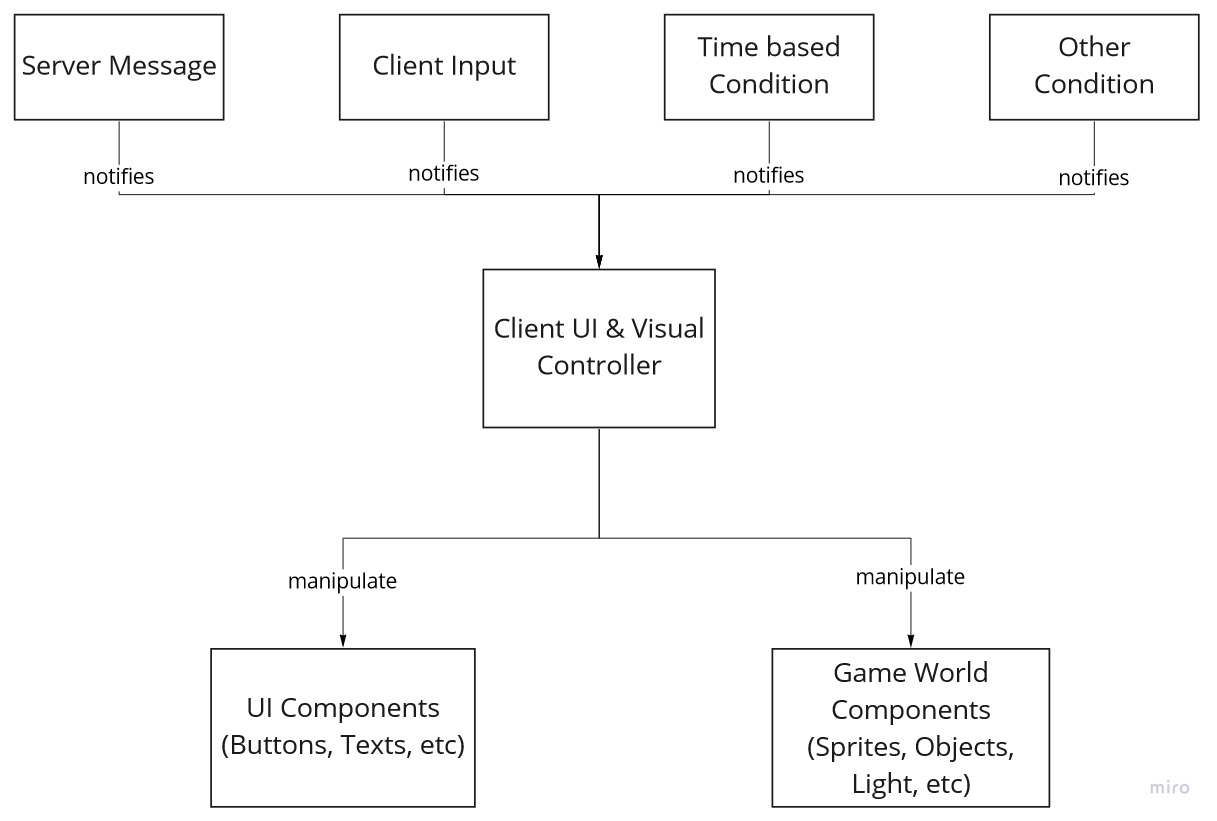
\includegraphics[width=150mm]{images/Client_UI_und_Visual_Konzept.jpg}
	\caption[Client UI \& Visual Controller Diagramm]{Veranschaulichung des Client UI \& Visual Controller Konzepts}
	\label{pic:Client_UI_und_Visual_Konzept}
\end{figure}

Wichtig ist, dass Funktionen des Client UI \& Visual Controller erst nach server- oder clientseitigen Überprüfungen ausgeführt werden. Der Controller selbst sollte nur überprüfen, ob fluktuierende Komponenten noch existieren oder sich in einem konsistenten Zustand befinden. Spiel-Relevante Logik, beispielsweise, ob ein Spieler berechtigt ist, bestimmte Aktionen durchzuführen, ist nicht Teil des Client UI \& Visual Controllers.

\section{Server Network Manager}

Der Server Network Manager ist für die korrekte Abarbeitung von serverseitigen Aufgaben zuständig, welche aufkommen, sobald ein Netzwerk-spezifisches Ereignis stattfindet.

\textbf{Beispiel:} \\
Die Verbindung eines Clients bricht mitten in der laufenden Spielszene ab. Der Server Network Manager stößt infolgedessen Funktionen anderer serverseitigen Manager-Komponenten an, welche dafür sorgen, dass alle Spieler über den neuen Zustand des Spiels informiert werden. Hierfür müssen zunächst serverinterne Variablen aktualisiert werden.

\textbf{Beispiel:}  \\
In einem Online-Ableger des Spiels 'Mensch ärger dich nicht' verliert ein Spieler seine Netzwerkverbindung. Als Reaktion kümmert sich der Server Network Manager darum, dass das Spiel trotzdem zu Ende gespielt werden kann. Die Spielfiguren des ausgeschiedenen Spielers müssen entfernt, und der Spiel-Fortschritt aktualisiert werden. Diese Funktionen stellt möglicherweise der \hyperref[spawn_manager]{Runtime Spawn Manager}, \hyperref[progress_manager]{Progress / Game State Manager } zur Verfügung.
Außerdem muss dem \hyperref[serverside_client_manager]{Serverside Client Manager} mitgeteilt werden, dass dieser Spieler nun nicht mehr Teil der Spiel-Session ist.

Die folgende Grafik illustriert die Aufgaben des Server Network Managers:

\begin{figure}[H]
	\centering
	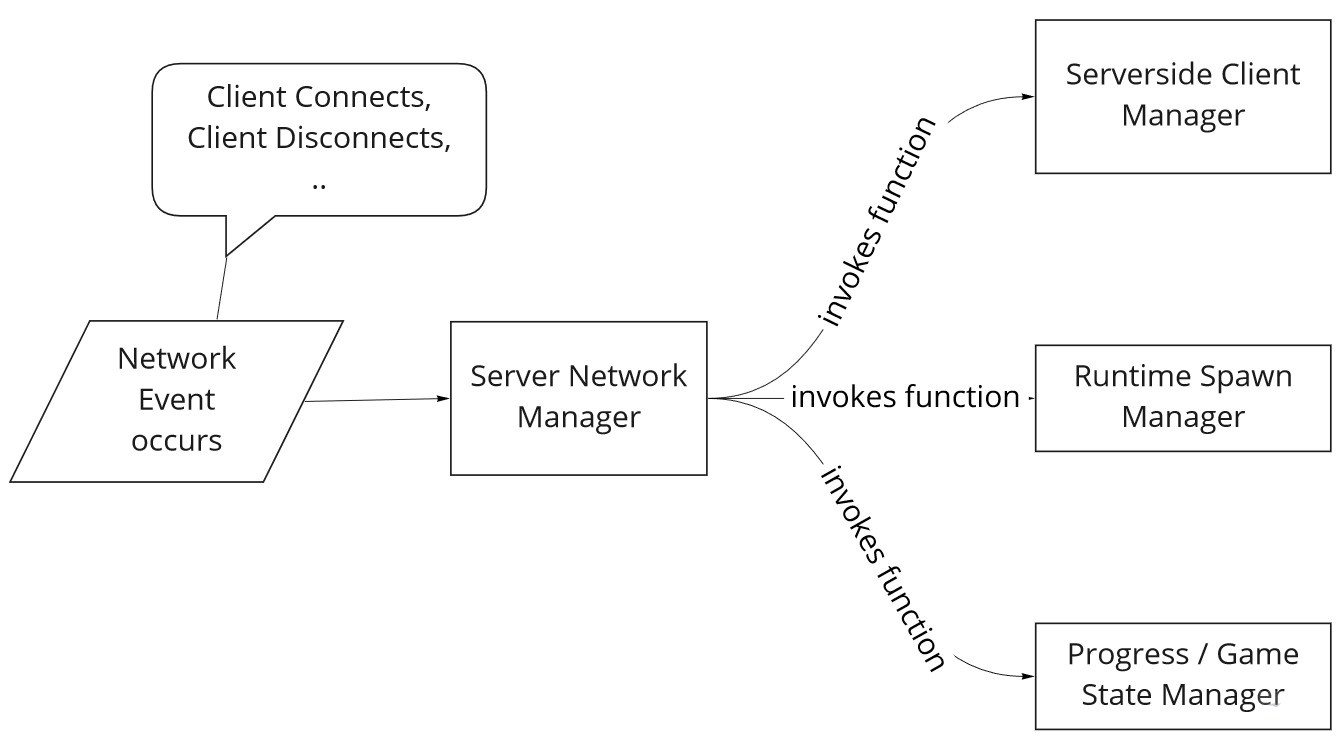
\includegraphics[width=150mm]{images/Server_Network_Manager.jpg}
	\caption[Server Network Manager Diagramm]{Veranschaulichung des Server Network Manager Konzepts}
	\label{pic:Server_Network_Manager}
\end{figure}

\section{Lobby / Multi Scene Manager}

Der Lobby/ Multi Scene Manager ist eine serverseitige Komponente, welche es erlaubt, Spielszenen-übergreifende Informationen zu speichern und zu verwalten. Beispielsweise könnte bei einem Lobby-basierten Matchmaking die Information des Leiters einer Lobby über Spielszenen hinweg gespeichert werden. Ebenso wäre es denkbar, dass der Bereitschafts-Status vor dem tatsächlichen Spiel innerhalb des Lobby / Multi Scene Managers gespeichert wird.

Außerdem stellt der Lobby / Multi Scene Manager Funktionen bereit, welche

- alle Clients informiert, sobald ein globaler Szenenwechsel angestoßen werden soll

- alle Clients über den aktuellen Status einer Lobby informiert.

\begin{figure}[H]
	\centering
	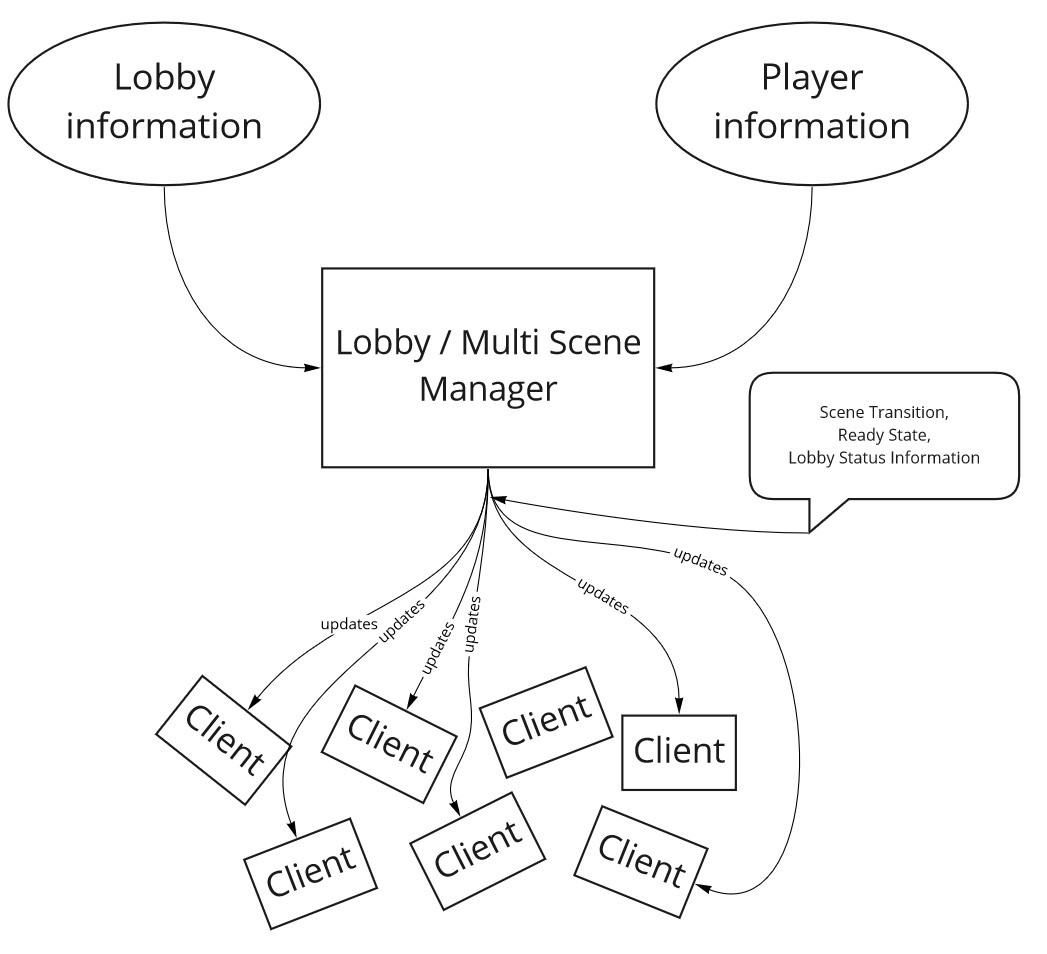
\includegraphics[width=150mm]{images/Lobby_Multi_Scene_Manager.jpg}
	\caption[Lobby / Mutli Scene Manager Diagramm]{Veranschaulichung des Lobby / Mutli Scene Manager Konzepts}
	\label{pic:Lobby_Multi_Scene_Manager}
\end{figure}


\section{Client Connection Manager}

Der Client Connection Manager beschreibt eine Softwarekomponente, welche folgende Aufgaben umsetzen muss:

- Implementierung von clientseitigen Methoden zum Informationsaustausch mit Matchmaking API.
Z. B. stellt die Matchmaking API dem Client über HTTP-Kommunikation Informationen bereit, mit denen sich der Client auf einen speziellen Server verbinden kann (IP + Port). \cite{Wikipedia.2021d} \cite{Wikipedia.2021e}

- Verarbeitung der von Matchmaking API bereitgestellten Informationen. 

Z. B. könnte die Matchmaking API einem Client die Information bereitstellen, dass aus einem bestimmten Grund dem angeforderten Serverbeitritt verweigert wird. Diese Information muss der Client Connection Manager zwischenspeichern und verwalten.

- Aufruf von Methoden eines Client UI Controllers.

Z. B. Die soeben erlangte Information über den verweigerten Serverbeitritt muss nun dem Nutzer dargestellt werden, hierfür ruft der Client Connection Manager Funktionen auf, welche ein Client UI Controller implementiert hat.

- Bereitstellung von Funktionen, welche den Beitritt zu einem Game-Server sicherstellen.

- Ausführen von Handler-Funktionen und Auslösen von Events für clientseitige Konsequenzen bei Netzwerkabbruch, manuellem Verlassen einer Server-Session oder sonstigen Abbruchgründen, welche dazu führen, dass eine Online-Spielsession verlassen wird.

Z. B. wird die notwendige Verbindung zum Internet während des Spiels unterbrochen. Der Client Connection Manager löst Callbacks aus, welche im Client UI \& Visual Controller implementiert sind. Diese sorgen dafür, dass der Spieler zurück ins Hauptmenü geleitet wird, in dem eine Fehlermeldung dargestellt wird, welche erklärt, warum das Spiel abgebrochen ist.

\begin{figure}[H]
	\centering
	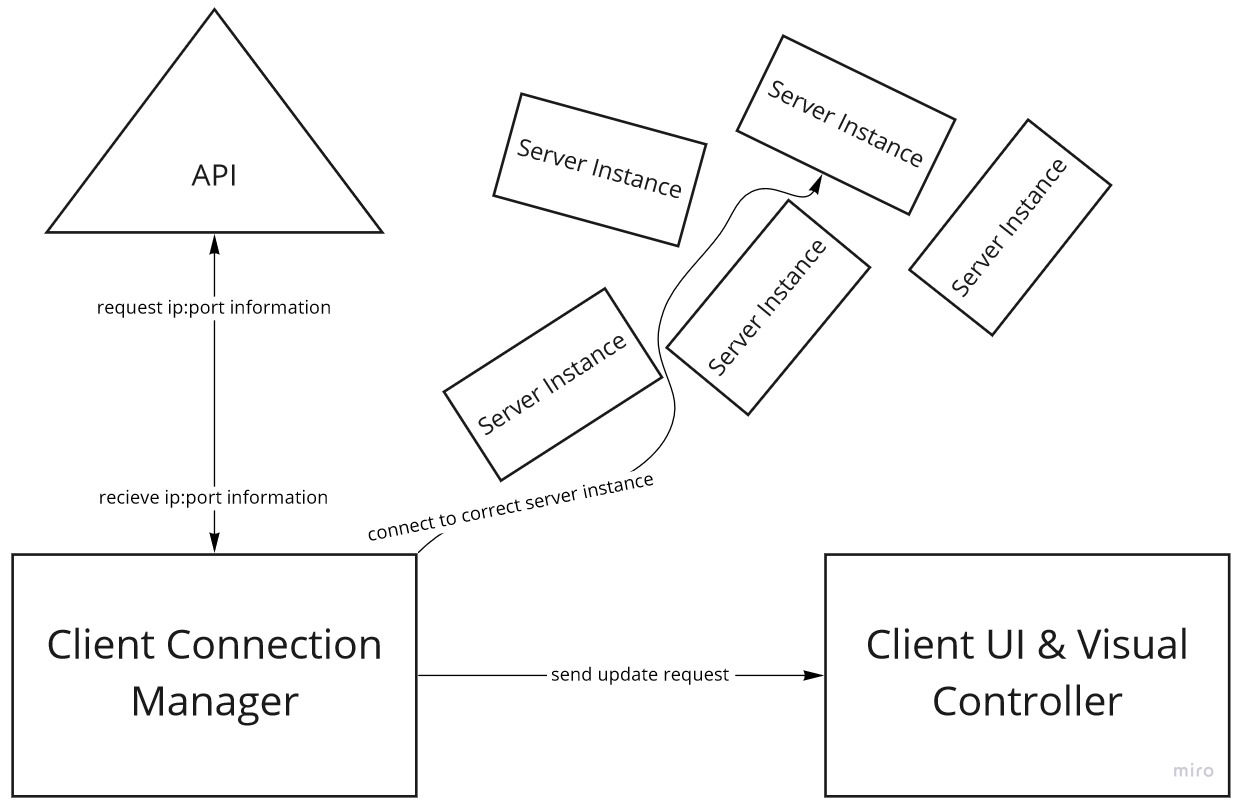
\includegraphics[width=150mm]{images/Client_Connection_Manager.jpg}
	\caption[Client Connection Manager Diagramm]{Veranschaulichung des Client Connection Manager Konzepts}
	\label{pic:Client_Connection_Manager}
\end{figure}

\section{Serverside Client Manager}

\label{serverside_client_manager}

Das Konzept des serverseitigen Client Managers beinhaltet die Verwaltung aller verbundener Clients innerhalb eines aktiven Serverprozesses. Insbesondere speichert der serverseitige Client Manager 2 Arten von Information über jeden Client:

Einerseits werden netzwerkbezogene Informationen über einen Client gespeichert, im einfachsten Fall ist dies lediglich die IP-Adresse des Hosts sowie der Port, auf welchem der Server seinen Kommunikationskanal geöffnet hat. Bei Spielkonzepten, welche eine weitergehende Authentifizierung des Spielers voraussetzen, können hier auch Benutzernamen, Benutzertags, E-Mail-Adressen o. ä. gespeichert und weiterverarbeitet werden.

Zum Anderen speichert und verwaltet der serverseitige Client Manager auch spielespezifische Informationen wie bspw. den aktuellen Anzeigenamen, konfigurierte Individualisierung des Spielcharakters, Spielerrollen oder andere Eigenschaften, über die der Server während einer Spiel-Session Kenntnis haben sollte.

Die folgende Grafik visualisiert diesen Informationsfluss:

\begin{figure}[H]
	\centering
	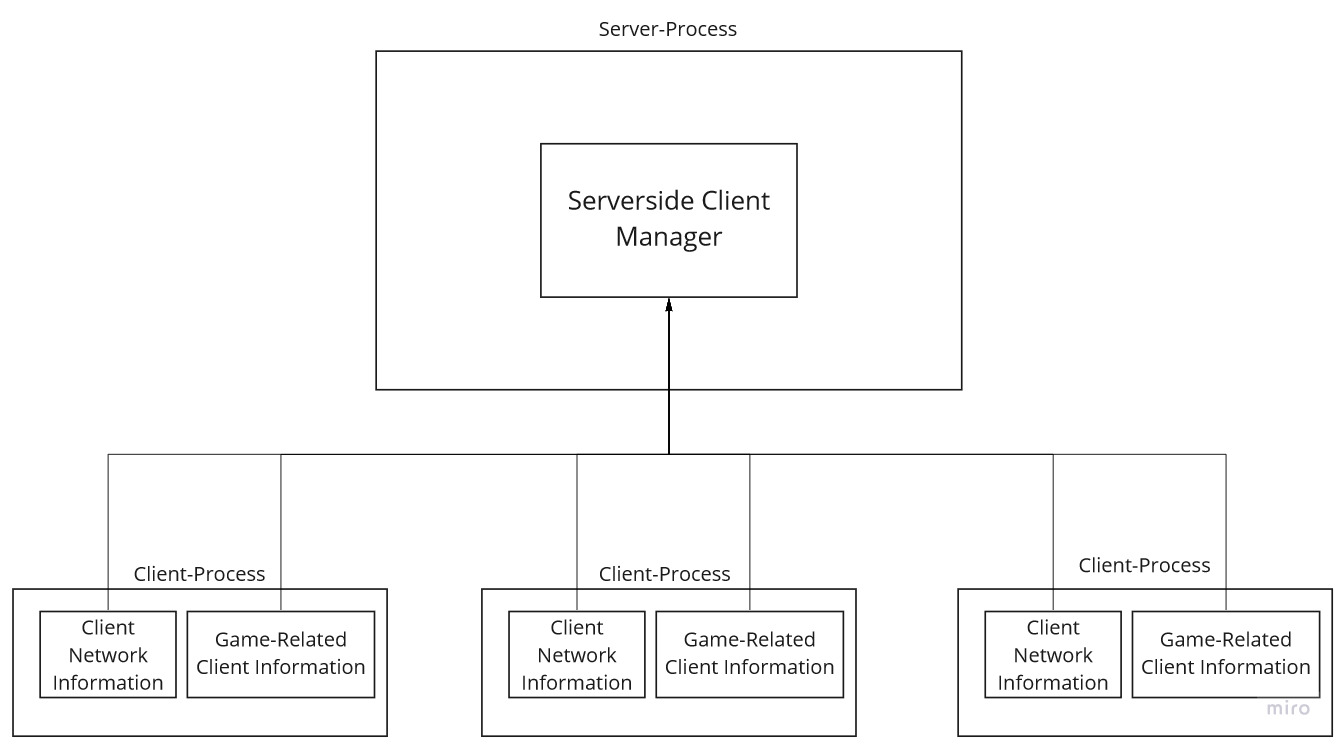
\includegraphics[width=150mm]{images/serversided_client_manager.jpg}
	\caption[Serversided Client Manager]{Veranschaulichung des serverseitigen Client Manager Konzepts}
	\label{pic:serversided_client_manager}
\end{figure}

\section{Prepare-Game-Manager}

Der Prepare-Game-Manager ist Teil des Serverprozesses und beinhaltet alle Funktionen, welche nötig sind, um eine Spielszene aufzubauen, bevor die Spieler ihr beitreten dürfen. Die Funktionen sollten konkret umsetzen:

- Spawning \cite{Wikipedia.2020} von NPCs \cite{Wikipedia.2021f} oder Spielgegenständen, die in Abhängigkeit zur Anzahl der beitretenden Spieler, einer Spielkonfiguration oder sonstigen Parametern stehen.

- Anpassung der Eigenschaften von bereits gespawnten NPCs oder Spielgegenständen, die in Abhängigkeit zur Anzahl der beitretenden Spieler, einer Spielkonfiguration oder sonstigen Parametern stehen.

- Initialisierung der Spawnpunkte für Spieler anhand von Spawnalgorithmen oder festgelegten Punkten in der Spielwelt.

- Abarbeitung sonstiger serverseitigen Abläufe, welche Voraussetzung für den Start des Spiels sind

Das folgende Diagramm zeigt, wann der Prepare-Game-Manager bei einem lobby-basierten Spielkonzept zum Einsatz kommt:

\begin{figure}[H]
	\centering
	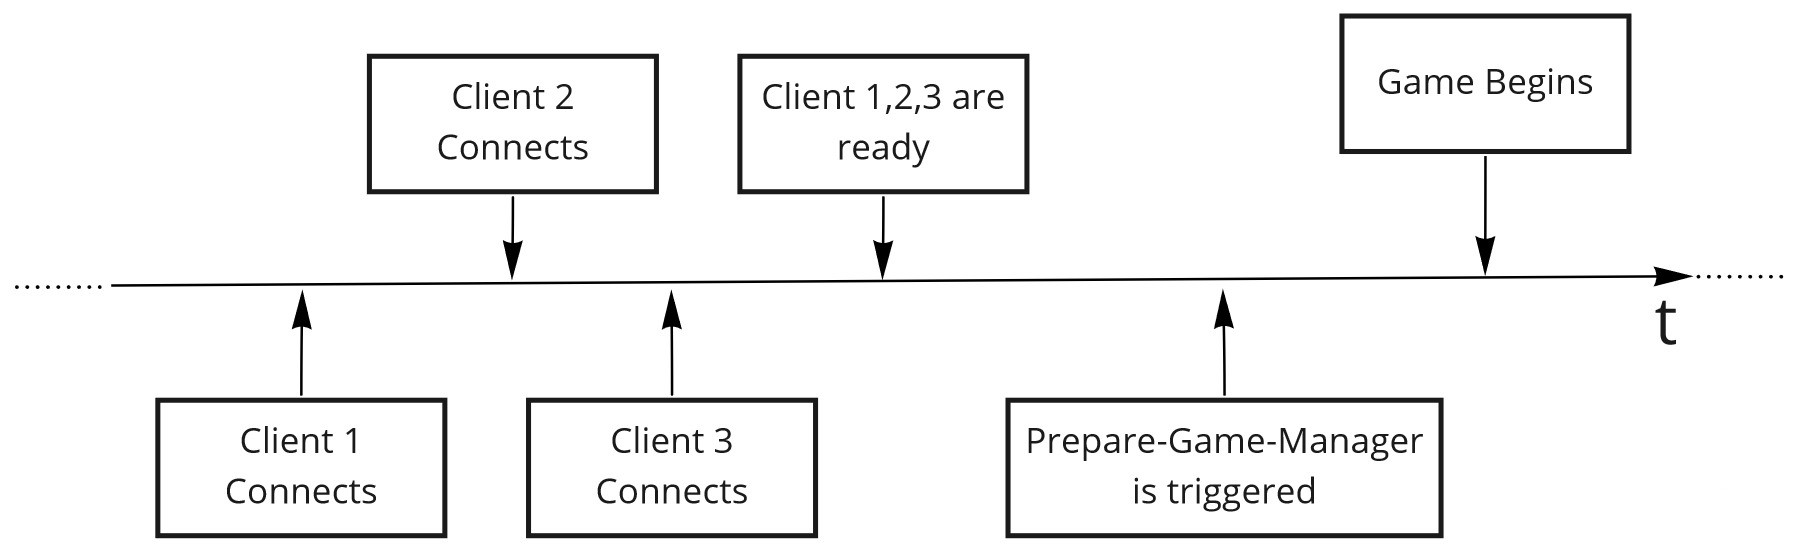
\includegraphics[width=150mm]{images/prepare_game_manager.jpg}
	\caption[Prepare-Game-Manager]{Veranschaulichung des Prepare Game Manager Konzepts}
	\label{pic:prepare_game_manager}
\end{figure}

\section{Progress / Game-State Manager}
\label{progress_manager}

Die Aufgabe eines Progress bzw. Game-State Managers ist es, Gewinn- bzw. Verlustbedingungen einer Spielsession zu speichern und zu verwalten. 

Beispiele hierfür sind: \\
- Verwaltung und Synchronisierung von globalen Timern
- Verwaltung und Synchronisierung von Spiel-Kennzahlen bzw. Variablen (z. B. der Spielstand bei einem Fußball-Match)

Außerdem ist der Progress Manager / Game-State Manager dafür verantwortlich, alle Clients über spielentscheidende Ereignisse zu informieren. 

Die Abfolge dieser Ereignisse werden im folgenden Diagramm aufgezeigt:

\begin{figure}[H]
	\centering
	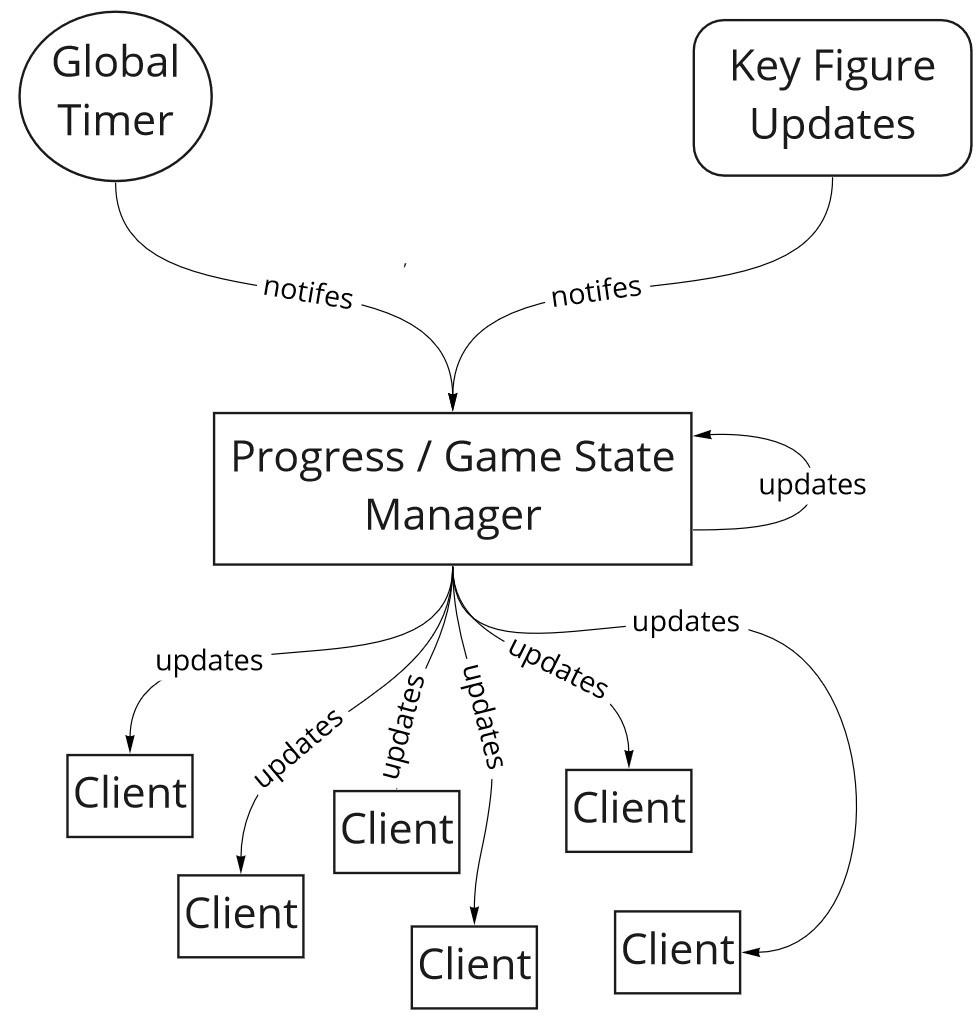
\includegraphics[width=150mm]{images/Progress_State_Manager.jpg}
	\caption[Progress / Game-State Manager]{Veranschaulichung des Progress / Game-State Manager Konzepts}
	\label{pic:Progress_State_Manager}
\end{figure}

\section{Runtime Spawn Manager}
\label{spawn_manager}

Der Runtime Spawn Manager verwaltet die zur Laufzeit zu erzeugenden Spieler- und Nicht-Spieler-Objekte. Konkret werden Funktionen des Runtime Spawn Managers ausgeführt, wenn ein spezifisches Event innerhalb einer Spiel-Session ausgelöst wird oder ein Spieler- bzw. Nicht-Spieler-Charakter stirbt, und diese erneut an anderer Position spawnen sollen ('Re-Spawning'). Die Logik, wo genau ein Spieler oder Nicht-Spieler Objekt seine neue Einstiegsposition erhält, regelt ebenfalls der Runtime Spawn-Manager.

\begin{figure}[H]
	\centering
	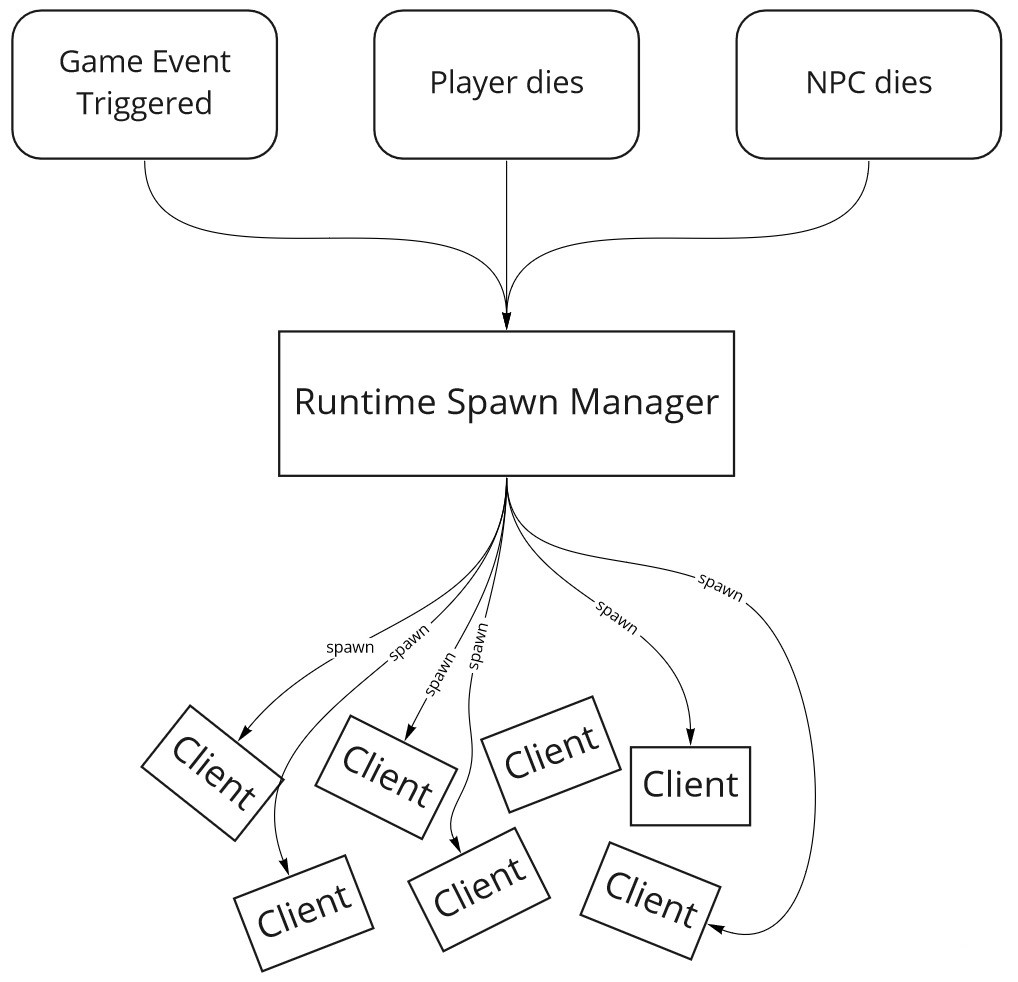
\includegraphics[width=150mm]{images/Runtime_Spawn_Manager.jpg}
	\caption[Runtime Spawn Manager]{Veranschaulichung des Runtime Spawn Manager Konzepts}
	\label{pic:Runtime_Spawn_Manager}
\end{figure}

\textbf{Beispiel:} In einem Online Multiplayer Ego-Shooter \cite{Wikipedia.2021g} stirbt ein Spieler durch Schüsse anderer Spieler. Der Runtime Spawn Manager sorgt dafür, dass anhand von bestimmten, zur Laufzeit ausgerechneten Bedingungen eine neue Spawn-Position für den gestorbenen Spieler gefunden wird. 


\section{Interest Manager}

Der Interest Manager kümmert sich um die Sichtbarkeit von Objekten. Wie bereits in der Sektion über \hyperref[interest_management]{Interest Management} erklärt, ist es je nach Spielkonzept notwendig, dass der Spieler stets nur über den für ihn relevanten Teil der Spielwelt Kenntnis hat. Aus diesem Grund sollten sich angehende Spieler-Entwickler fragen, ob sie eine solche Software-Komponente in die Architektur ihres Projekts integrieren möchten. Die folgende Grafik veranschaulicht diese Aufgabe:

\begin{figure}[H]
	\centering
	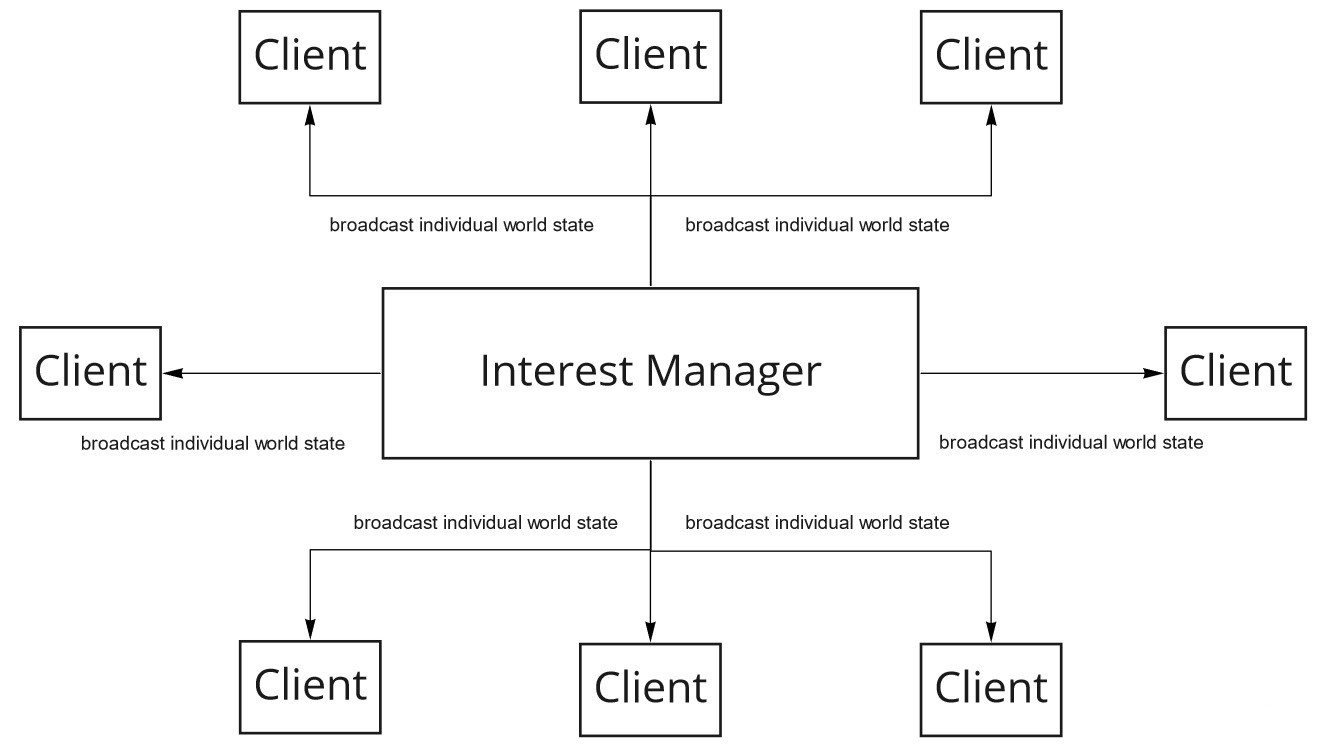
\includegraphics[width=150mm]{images/Interest_Manager.jpg}
	\caption[Interest Manager]{Veranschaulichung des Interest Manager Konzepts}
	\label{pic:Interest_Manager}
\end{figure}

Mögliche Faktoren, die der Interest Manager benutzen kann, um den Spielern die Objekte anzeigen zu lassen, die sie sehen dürfen sind:

- Distanz zwischen Spieler und anderen Objekten

- Teams bzw. Gruppen. Die registrierten (Spieler)-Objekte innerhalb eines Teams/ einer Gruppe sind für Spieler, welche ebenfalls innerhalb des Teams/Gruppe registriert sind sichtbar.

- Spatial Hashing / Grid Checker: Die Spielwelt und ihre Objekte werden in quadratische Zellen eingeteilt. Je nachdem in welcher Zelle sich ein Spieler befindet, werden nur diejenigen Objekte der Spielwelt mit dem Spieler synchronisiert, welche sich innerhalb der 8 'Nachbarzellen' befinden:

\begin{figure}[H]
	\centering
	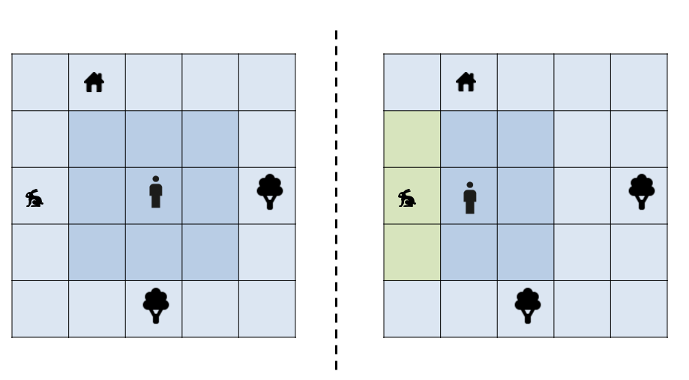
\includegraphics[width=150mm]{images/interest_management.png}
	\caption[Spatial Hashing]{Illustration des Interest Management Konzepts Spatial Hashing. \cite{JeromeRenaux.2017} }
	\label{pic:interest_management}
\end{figure}

Sollte keine der hier beschriebenen Beispiele auf das gewünschte Spielkonzept passen, so ist es notwendig, eine komplett eigene Logik für das Interest Management zu implementieren.
